\documentclass[a4paper]{article}
%\documentclass{report} % Can be article, report, book, anything you want!
\usepackage{csquotes}
\usepackage{float}
\usepackage{vub} % this will automatically set to A4 paper. We're not in the US.
% if, for some obscure reason, you need another format, please file an issue (see further).

% The `vub` package has many options.
% Please read the documentation at https://gitlab.com/rubdos/texlive-vub if you want to learn about them.

% Feel free to mix and match with other packages.
\setlength\parskip{\baselineskip}
\title{A small report about the project}
\subtitle{Security in Computing}
\faculty{Sciences and Bio-Engineering Sciences} % Note: without the word "Faculty"!
\author{Gérard Lichtert}
\date{\today}

\begin{document}
\maketitle
\raggedright{}
\tableofcontents%
\newpage
\section{Overview \& Implementation of requirements}
The functionalities of the application have not decreased with regards to what the user is able to do within the client. A user can still do the following interactions with the application:
\begin{itemize}
    \item Login a user
    \item Send a message to a room or a direct room
    \item Create a room, public or private
    \item Join a public room
    \item Add a user to a private room
    \item Leave a room
\end{itemize}
However, now a user also has to register themselves prior to being able to login to the application. This is because users are no longer saved in memory but in a database. Which we will discuss in after the next subsection, because this belongs to the persistance requirement.

\subsection{Login / Authentication}
For the registration of users, the client sends a request to the server to register a user. The password is hashed using bcrypt as the hashing library which also uses salt to hash the password, before being stored in the database. Note that the user is only registered if the user does not already exist. Otherwise a pop up will notify the user already exists.

For the login of users, the server fetches the user credentials from the database. Then the server compares the plaintext password against the hashed password using bcrypt. If the password is correct, the server will generate a JSON Web Token (JWT) using the HS512 algorithm and signing it with the private key of the server, which you'll have to generate and store to a .env file (more below). The JWT will be sent back to the client, which will be stored in a variable on the client. The JWT will be used to authenticate the user for the rest of the session, as the rest of the interactions with the server require a valid JWT. Interactions with the server done without the JWT or with invalid JWT will be rejected by the server.

\subsection{Persistence}
In the skeleton application all of the details regarding, messages, information about rooms or even users were all stored in-memory. Now it is stored in a sqlite3 database, which is a file-based database. While not ideal for production, it is a good alternative for a school project as it maintains the aspects of a relational database without the need for a hosting service of the database. Ideally I would choose something like a MySQL or PostgreSQL database for a production environment. Note that the database is not supplied when first downloading the application, but when the server is started for the first time, the database will be created, if it does not already exist. To prevent SQL injection, the interactions with the database all use prepared statements.
The database structure is as follows:
\begin{figure}[H]
    \centering
    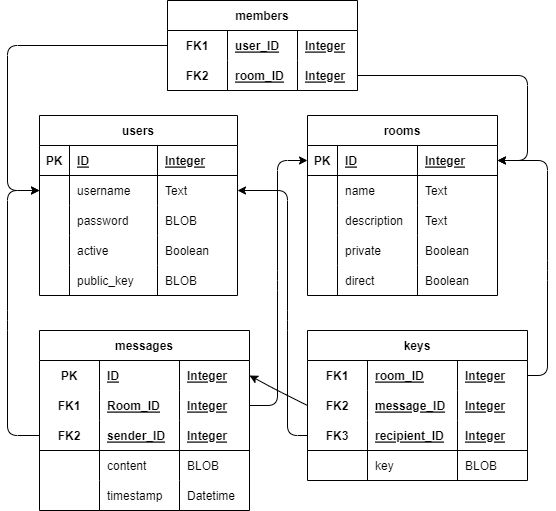
\includegraphics[width=0.7\textwidth]{database.png}
    \caption{The database structure}
\end{figure}
We have a table denoting the users, in which their username, hashed password and public keys are stored and an ID is generated.

We have a table denoting the rooms, in which the room name, the room description and wether the room is private or direct is stored as well as a room ID is generated.

To link users to rooms, the database has a table called members, which references the room ID and the user ID, linking a user to a room. These combinations are also unique, so a user can only be in a room once.

To store the messages we also have a messages table, which stores the message, the user ID of the sender and the room ID of the room the message was sent in. When the message is stored, it automatically creates a timestamp and ID for the message.

To store the decryption keys\footnote{These are encrypted} of the encrypted messages, we have a table called keys, which stores the room ID, message ID, (both referencing the message and room tables), the decryption key as well as the user ID of the user who is able to decrypt the message. This is to ensure that only the user who is allowed to decrypt the message can decrypt the message. Perhaps not irrelevant to mention is that, only the users who are in the room where the message was sent, have a key stored in the database, therefore if a user is not in the room, they will not be able to decrypt the message.

\subsection{End-to-end encryption}
To implement e2e encryption I used the native crypto library of node.js. Upon attempting to register a user a RSA key pair is generated. The public key is sent along the registry details and when the registration is successful, the private key is stored on the client. The public key is stored in the database.
For e2e encryption we have two scenarios:
\begin{itemize}
    \item A user sends a message to a direct room (a room with only two users, the amount of users can never change)
    \item A user sends a message to a private room (a room with a variable amount of users)
\end{itemize}
\subsubsection{Sending a message to a direct room}
When sending a message to a direct room, the sender will generate a symmetric AES Key and an IV. The message is encrypted using the AES key and the IV followed by prepending the IV to the message. The AES key itself is then encrypted with the recipients public key, which is obtained from the server from the database. The message is sent to the server and stored in the database. It is then broadcasted to the room that there is a new message. When the recipient opens the room with the sender, it will receive the message as well as the encrypted AES key. The recipient can now split the message, extracting the IV and the encrypted message, decrypt the encrypted AES key with the recipients' private key and decrypt the message with the IV and AES key. The message can now be displayed on the clients user interface (UI).

Note that a new AES key and IV is generated for each message.

Important to know is that the sender also encrypts the AES key with the senders' public key. This means that in direct rooms there will be 2 encrypted AES keys stored per message. This is done because the sender also needs to be able to read the message, and thus decrypt it with his or her private key.
\subsubsection{Sending a message to a private room}
While sending a message to a private, the process is not very different from sending messages to a direct room. For each message a AES key and IV is generated, the message is encrypted with the AES key. The difference lies in how many times the AES key is encrypted. In a direct room you essentially have two encrypted AES keys, one for the sender and one for the recipient, since there are two members in a direct room. However, in a private room, we can have an arbitrary number of members, say \(n\) members. This means that the AES key has to be encrypted \(n\) different times, once for each recipient + the sender. Consequently, each message will generate \(n\) encrypted AES keys. Note that it is the same AES key.The decryption process stays the same.

To prevent removed users from being able to read the messages, we implement a few protection layers. One is that the user will never receive messages from the server regarding the left room. Two is that the sender will never generate an encrypted AES key for the removed user, making it nearly impossible for the removed user to decrypt the AES key without the recipients private key. Lastly, if the user happens to rejoin the room after the user left, the database will only fetch the messages for which the user has a encrypted AES key to decrypt the messages in the room. Meaning that the database will never return the messages that were sent in the period that the user was not part of the room.

\subsection{Client-side security}
To protect the client from html injection as well as XSS attacks, I used the sanitize-html and validator libraries. The sanitize-html allows for the removal of html tags, even if they need to be concatenated. The validator, validates inputs, as well as removes illegal characters from inputs, which is the case when registering or logging in. Only alphabetical characters and numbers are allowed. This does lead to a less secure password for the users, since there are less characters to pick from.

When creating a room, a user needs to input the room name as well as the description. Both are sanitized for html tags, as they are not needed in these fields.

When interacting with the client, one could change the HTML to mess with the interactions. However, these interactions are validated with their expected datatype. If the datatype does not match, the client will not allow the interaction.

Furthermore, messages are only escaped, as it might be useful to send messages discussing html tags. In which case removing the html tags would be an issue rather than a solution.

\subsection{Dependency management}
Upon starting the project I ran \enquote{npm audit} to detect issues with libraries. I don't exactly remember if there were any but when I ran \enquote{npm update} regardless, to update all dependencies, I did notice some deprecated packages. Regardless all the packages are now up to date on both clients and server.
\section{Security goals and attacker models}
The security goals of the application were to mitigate the passive network attackers models and part of the web attacker. The passive network attacker model is mitigated by the use of e2e encryption on private or direct channels. While the attacker can eavesdrop on the channels, it cannot read the messages unless the attacker has a recipients private key. The web attacker model is mitigated by having a desktop application, making the user use a certified front-end, instead of a browser application which can be spoofed or tampered with. However, it is still possible for attackers to attempt XSS injection in the clients' inputs, which is why the public part of the client forwards the data to the non-public part, where inputs are sanitized and validated. Before the data is sent to the server.

\section{Description of important cases and design choices}
When data is sent to the server, it is currently assumed to be sanitized and validated by the client. However, there are still attacks possible to the database, through sql injection. This is why all interactions with the database are done through prepared statements, to prevent sql injection.

Another design choice, which was mentioned earlier, is the way that messages are returned from the database. The database will only return messages for which the user has a decryption key. This is to prevent users who are not in the room from being able to read the messages that were sent while the user was not in the room.

For the encryption of e2e encryption, the sender of the message generates a symmetric AES key and IV. Encrypts the message with the symmetric key and the symmetric key with the recipients public key. To protect public messages they are encrypted with the servers' public key. The server decrypts it with its private key to store it in the database. When a user fetches the public messages, the server encrypts the messages with a symmetric AES key, which is encrypted by the users' public key. This way only the user can decrypt the messages.

The passwords are hashed with bcrypt, which users salt to hash the password. This way the passwords are illegible to anyone who has access to the database.
\section{Manual on how to run and test the application}
\subsection{The server}
To run the server, you require node.js of version 20.11.1 or higher. First it is required to create a .env file in the directory. In the .env file you should create a variable called \enquote{SECRET\_KEY}. The value that should be assigned to this is a key generated by executing the command \enquote{openssl rand --base64 512}. As an example:
\begin{figure}[H]
    \centering
    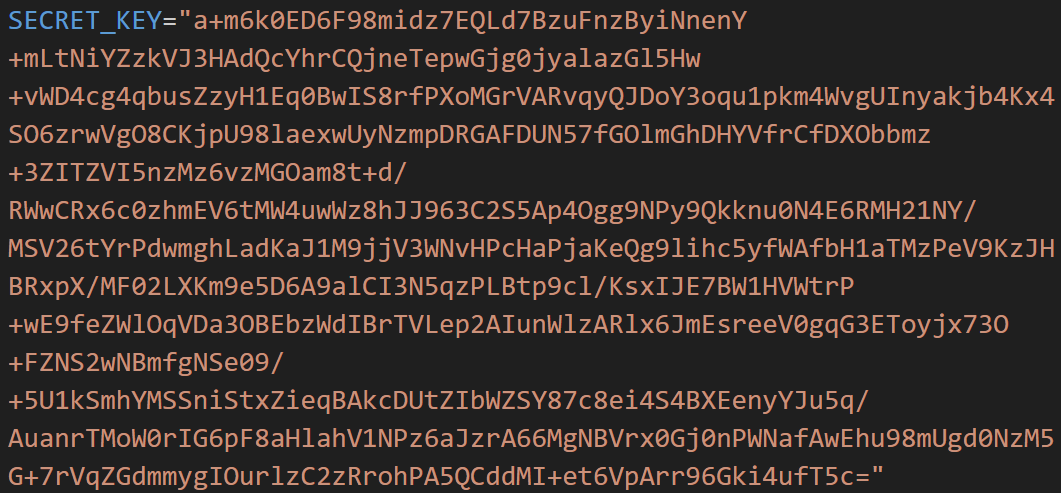
\includegraphics[width=0.6\textwidth]{openssl.png}
\end{figure}
After creating the .env file and storing a secret key in the file, it should be sufficient to run \enquote{npm install} to install the dependencies and \enquote{npm start} to initialize the database, if it is not present and the server itself, as well as create the key pair for the server. 
\subsection{The client}
To run the client, you require node.js of the same version as the server. It should be sufficient to run npm install followed by npm start to run the client. The client will automatically create a directory to store private keys and display the UI.
If the database was not present during the start of the server, the user will first have to register. After logging in the user will be able to use the functionalies mentioned in section 1.
\section{Added dependencies}
\subsection{Client}
The following depenencies were added to the client:
\begin{itemize}
    \item validator
    \item sanitize-html
    \item nodemon
\end{itemize}
\subsection{Server}
The following dependencies were added to the server:
\begin{itemize}
    \item bcrypt
    \item sqlite3
    \item jsonwebtoken
    \item dotenv
    \item sqlite3
\end{itemize}
\end{document}
